	This first step requires correctly placing any edge with white; this completes the `cross' on the white face and aligns the edges appropriately. This results in the configuration shown in \figref{topcross}.
\begin{figure}[h]
	\centering
	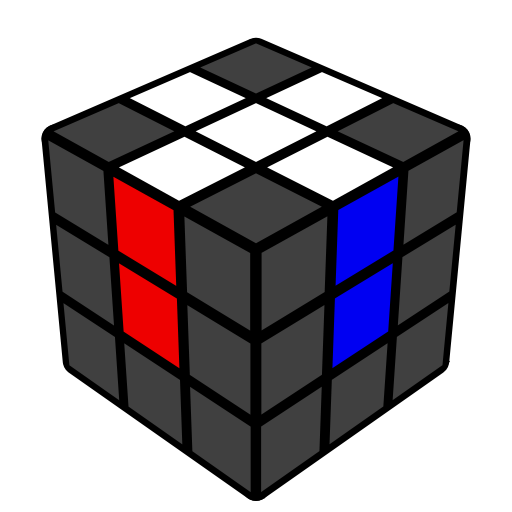
\includegraphics[width=0.3\textwidth]{topcross.png}
	\caption{Solved white cross}\label{fig:topcross}
\end{figure}

\begin{enumerate}
	\item \label{step:find} Find a white edge piece on the bottom layer.
	\item \label{step:align} Twist the bottom layer to align the piece you found with the corresponding non-white centre.
	\item Bring the piece to the top layer:\begin{enumerate}
		\item If the edge is already correctly aligned with the centre, twist it 180\degree , as seen in \figref{edgeup180}.
		\item Otherwise, twist it 90\degree to move it to the middle layer on a different face. Twist that new face to bring it back to the bottom layer. Then, go back to step~\ref{step:align}. This is shown in \figref{edgeup90}.
	\end{enumerate}
\begin{figure}[h]
	\centering
	\begin{subfigure}[b]{0.3\textwidth}
		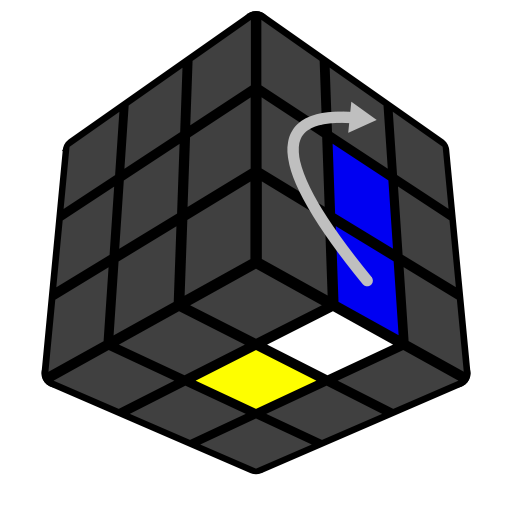
\includegraphics[width=\textwidth]{turn180.png}
		\caption{If aligned}{\label{fig:edgeup180}}
	\end{subfigure}
	\begin{subfigure}[b]{0.3\textwidth}
		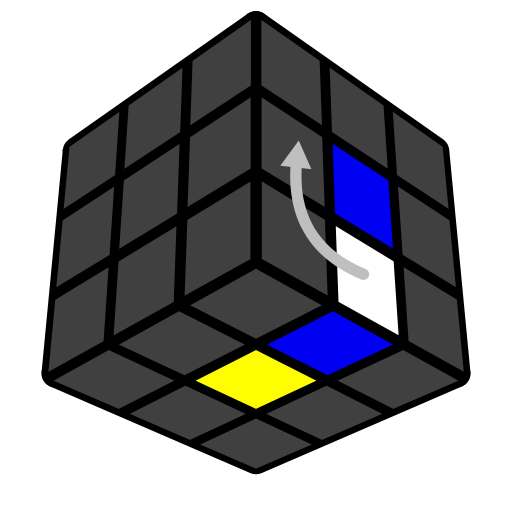
\includegraphics[width=\textwidth]{turn90.png}
		\caption{If not aligned}{\label{fig:edgeup90}}
	\end{subfigure}
	\caption{Bringing edges up}
\end{figure}
\newpage
	\item Repeat from step~\ref{step:find} until there are no more white edges on the bottom layer.
	\item Bring any white edges on the middle layer to the bottom layer by twisting 90\degree .
	\item Repeat from step~\ref{step:find} until there are no more white edges on the middle layer.
	\item Bring \emph{unsolved} white edges to the bottom layer by twisting 180\degree .
	\item Repeat from step~\ref{step:find} until the cross is complete.
\end{enumerate}

